%%%%%%%%%%%%%%%%%%%%%%%%%%%%%%%%%%%%%%%%%
% Stylish Article
% LaTeX Template
% Version 2.2 (2020-10-22)
%
% License:
% CC BY-NC-SA 3.0 (http://creativecommons.org/licenses/by-nc-sa/3.0/)
%
%%%%%%%%%%%%%%%%%%%%%%%%%%%%%%%%%%%%%%%%%

%----------------------------------------------------------------------------------------
%	PACKAGES AND OTHER DOCUMENT CONFIGURATIONS
%----------------------------------------------------------------------------------------

\documentclass[fleqn, 11pt]{SelfArx} % Document font size and equations flushed left

\usepackage[english]{babel} % Specify a different language here - english by default

\usepackage{array} % Required for centering tables content

\usepackage{float} % Avoid putting tables on top of the pages

\usepackage{subfig} % Put more subfigures in the same figures

\graphicspath{ {./images/} } % Paths were images are taken

%----------------------------------------------------------------------------------------
%	COLUMNS
%----------------------------------------------------------------------------------------

\setlength{\columnsep}{0.55cm} % Distance between the two columns of text
\setlength{\fboxrule}{0.75pt} % Width of the border around the abstract

%----------------------------------------------------------------------------------------
%	COLORS
%----------------------------------------------------------------------------------------

\definecolor{color1}{RGB}{0,0,90} % Color of the article title and sections
\definecolor{color2}{RGB}{0,20,20} % Color of the boxes behind the abstract and headings

%----------------------------------------------------------------------------------------
%	HYPERLINKS
%----------------------------------------------------------------------------------------

\usepackage{hyperref} % Required for hyperlinks

\hypersetup{
	hidelinks,
	colorlinks,
	breaklinks=true,
	urlcolor=color2,
	citecolor=color1,
	linkcolor=color1,
	bookmarksopen=false,
	pdftitle={Title},
	pdfauthor={Author},
}

\setlength{\parindent}{0cm} % Remove left padding from text

\newcolumntype{C}[1]{>{\centering\arraybackslash}p{#1}} % centering columns values

%----------------------------------------------------------------------------------------
%	ARTICLE INFORMATION
%----------------------------------------------------------------------------------------

\JournalInfo{\today} % Journal information
\Archive{\textcopyright \space 2022} % Additional notes (e.g. copyright, DOI, review/research article)

\PaperTitle{Implementation of a DoS attack exploiting mDNS} % Article title

\Authors{A. Al Masoud • F. Amato • A. Blindu • D. Lotito • D. Ragusa} % Authors
\affiliation{\textit{Department of Computer Engineering, University of Pavia, Pavia, Italy}} % Author affiliation
\affiliation{\textit{Enterprise Digital Infrastructure}} % Author affiliation

\Keywords{\small{DoS • mDNS • Security • LAN }} % Keywords - if you don't want any simply remove all the text between the curly brackets
\newcommand{\keywordname}{Keywords} % Defines the keywords heading name

%----------------------------------------------------------------------------------------
%	ABSTRACT
%----------------------------------------------------------------------------------------

\Abstract{The aim of this report is to discuss an implementation of a DoS attack, on a local area network (LAN), exploiting the mDNS protocol. 
The generated traffic has been analyzed and some studies have been conducted to understand the impact of this attack under many conditions.
Moreover, other possible vulnerabilities of this protocol, and some possible countermeasures that can be implemented to overcome these security issues, have been identified.}

%----------------------------------------------------------------------------------------

\begin{document}

\maketitle % Output the title and abstract box

\tableofcontents % Output the contents section
\vfill\null

\thispagestyle{empty} % Removes page numbering from the first page

%----------------------------------------------------------------------------------------
%	INTRODUCTION
%----------------------------------------------------------------------------------------


\section{Introduction} % The \section*{} command stops section numbering
The core of this project is to implement a DoS attack, exploiting the mDNS (Multicast Domain Name System) protocol \cite{rfc6762}, used for making various types of devices communicate each other, on a local area network, this to show how easily inaccessible the service can be. \newline

In general, a DoS attack is when an attacker attempts to make impossible for a target to provide a service, or a set of services. These attacks, in general, work by overwhelming a system with requests for data. \newline
This goal is usually achieved by sending small requests to a third party service, spoofing the IP address of the source of the requests with the target's one, and the third party service sends bigger responses to the target's requests, letting it crashing. \newline 
The result is that the available bandwidth and target's resources become overloaded.\newline
In this project, the mDNS protocol has been used because it allows \textit{amplification}, by exploiting particular types of queries that send a lot of data ({\it{ANY}} type), and also \textit{reflection}, sending packets to all devices in the network through the multicast mode. \newline

To simplify the work, an initial assumption has been established: the attacker and the target devices are connected within the same network although, as will be explained below, the attack can also come from the outside in case of misconfiguration.

%----------------------------------------------------------------------------------------
%	mDNS protocol
%----------------------------------------------------------------------------------------

\section{The mDNS protocol}
Multicast DNS (mDNS) is a service aimed to solve name resolution problem in smaller networks. It takes a different approach with respect to the well-known DNS: instead of sending requests to a name server, the network participants are all contacted through multicast mode. \newline
Instead, a similarity to the classic DNS protocol is that mDNS is an application layer protocol (considering the TCP/IP network stack) that relies on top of the UDP protocol. \newline

A client, that needs to know information about an hostname, sends a query to all the devices in the network. The response, instead, should go to the entire network or directly to the client in unicast. In this way, if the answer is sent to all devices in multicast, all of them are informed about the name and IP address such that they can create an entry in their mDNS cache. \newline
Multicast DNS can cause relatively high traffic, so the protocol actively tries to conserve network resources: to this end, the requesting client sends the correct response according to its opinion (i.e. according to the current cache entry). Only if this is no longer correct, or if the entry is about to expire, the recipient have to respond. \newline
Generally, only hostnames ending with {\it{.local}} can be used with Multicast DNS.
\begin{figure}[H]\centering
    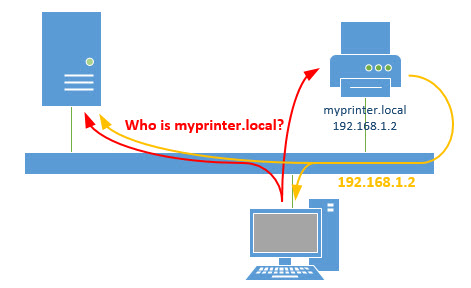
\includegraphics[width=\linewidth]{./mdns-02.jpg}
    \caption{Example of mDNS operation where the query (red) is sent to all devices and the same happens for the response (yellow) from the printer}
    \label{fig:msdns-1}
\end{figure}

The mDNS has been developed in the Zeroconf (Zero Configuration Networking) context, by using the same programming interfaces and operating semantics as the standard unicast Domain Name Service (DNS). 
The idea of Zeroconf is allowing computers to communicate with each other without the need for a prior configuration.\newline

A popular implementation of mDNS is \textit{Bonjour} by Apple, but also the open source software \textit{Avahi} can be used as an mDNS service. It is also available for Windows OS (after version 10).

\paragraph{Advantages} 
\begin{itemize}[leftmargin=*]
    \item Since all devices share their IP addresses, there is no need to configure a server or directory. This makes it possible to add additional devices very dynamically and quickly.
\end{itemize}

\paragraph{Disadvantages} 
\begin{itemize}[leftmargin=*]
    \item Although the protocol tries to keep network traffic low, participating computers must constantly monitor the network and process incoming messages. This requires computing power.
    \item Assigning host names is problematic: since it can be freely choosen a name for each device, as long as it ends in {\it{.local}}. This can lead to two network devices with the same host name. The developers of mDNS have deliberately not proposed a solution to this problem: on the one hand, it is assumed that the case rarely occurs; on the other hand, the double naming may be intentional. \newline 
    mDNS resolves ending with the {\it{.local}} top-level domain (TLD) hostnames. This can be a possible source of problems, if {\it{.local}} includes hosts that do not implement mDNS, but can be found via an unicast DNS server. Resolving this conflicts requires network configuration changes, that mDNS prefers avoiding.
    \item In some cases, mDNS is open. This means that it also responds to requests from outside (the Internet). Attackers can find such open services and use them for DoS attacks, using network devices improperly. \newline
    In addition, using mDNS, even sensitive data can be detected. This allows attackers to know information about connected devices and use it for further attacks.
\end{itemize}

\subsection{Packets structure}
An mDNS message is a UDP packet sent in multicast using the following addressing:
\begin{itemize}[leftmargin=*]
    \item IPv4 address \textit{224.0.0.251} or IPv6 address \textit{ff02::fb}
    \item UDP port \textit{5353}
\end{itemize}
The mDNS payload structure is based on the unicast DNS packet format, which consists of two parts: the header and the data.\newline
The header, shown in Figure \ref{fig:msdns-message-1}, is identical to the one in unicast DNS, as the subsections in the data part, composed of: queries, responses, authoritative-nameservers, and additional records.
\begin{figure}[H]\centering
    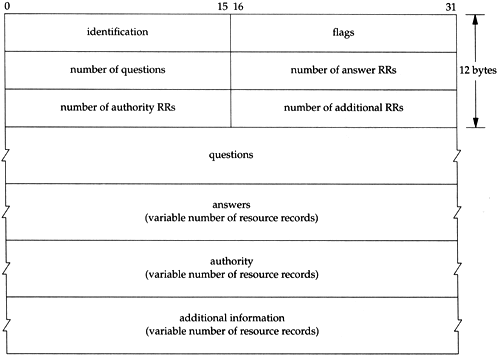
\includegraphics[width=\linewidth]{./msg-format.png}
    \caption{mDNS/Unicast DNS message format}
    \label{fig:msdns-message-1}
\end{figure}

\subsection{Queries}
The format, shown in Table \ref{tab:query-section}, of the query section is a bit different from that of the classic DNS because it adds a single-bit {\it{"QU" question}} field. \newline

\begin{table}[hbt]
	\centering
	\begin{tabular}{|C{2cm}|C{2.8cm}|C{1.5cm}|}
		\hline
		\textbf{Field} & \textbf{Description} & \textbf{Length} \\
		\hline
		\hline
		Name & Name of the node & Variable \\
		\hline
		Type & The type of the query & 16 \\
		\hline
		Class & IN & 15 \\
		\hline
		"QU" question & Boolean flag indicating whether a unicast response is desired & 1 (higher order bit of Class field)\\
		\hline
	\end{tabular}
	\caption{Query section fields}
	\label{tab:query-section}
\end{table}

The {\it{Class}} field is identical to that found in unicast DNS ({\it{IN}} class).
The {\it{"QU" question}} field is used to minimize unnecessary transmissions over the network: if the bit is set (the high order bit of the Class field), responders should send a direct-unicast response to the requesting node rather than broadcasting the response to the entire network.\newline

\subsection{Resource Records}
All records in the answers, authoritative-nameservers, and additional records sections have the same format while the RRs in the answer section in mDNS are slightly different from classic DNS. What they are and their length are shown in Table \ref{table}. \newline

In particular, the {\it{Cache-flush}} bit is used to instruct neighboring nodes that the record should overwrite, rather than be added to any existing cache entry for this RR {\it{Name}} and {\it{Type}}.

\begin{table}[hbt]
	\centering
	\begin{tabular}{|C{2.0cm}|C{4.2cm}|C{1.25cm}|}
		\hline
		\textbf{Field} & \textbf{Description} & \textbf{Length} \\
		\hline
		\hline
		Name & Name of the node & Variable\\
		\hline
		Type & Type of the Resource Record & 16\\
		\hline
		Class & Class code, 1 also known as IN for the Internet and IP networks & 15\\
		\hline
		Cache-flush & Boolean flag indicating whether outdated cached records should be purged & 1\\
		\hline
		TTL & Time interval (in seconds) RR should be cached & 32\\
		\hline
		Data length & Integer representing the length (in octets) of the RDATA field & 16\\
		\hline
		Data & Resource data; internal structure varies by RRTYPE & Variable\\
		\hline
	\end{tabular}
	\caption{Resource Records}
	\label{table}
\end{table}

%----------------------------------------------------------------------------------------
%	Tools used
%----------------------------------------------------------------------------------------

\section{Tools used}
Several tools have been used during the experiment, some of them developed in-house. In this section, they are presented and their source can be analyzed in the Github repository \cite{mDNS-security}. 

Moreover, a {\it{Python Jupyter notebook}}, not described in this report, has been used to perform analysis of the data collected during the experiments (plotting graphs).

\subsection{Scripton.py}
\textit{Scripton} is a Python script that is used during the experiment to send thousands of query packets in multicast, thus allowing the actual DoS attack to be carried out.
In this sense, multithreading is exploited so that packets can be sent massively. The payload of each query, instead, is built, in hexadecial code, in the \textit{build\_message()} function making use of the specification defined in the RFC\cite{rfc6762}. Each packet is then sent directly in multicast from a socket avoiding intermediate services that could slow down the attack by waiting for a response from the mDNS service.

Scripton can also spoof an IP in the network by acting on the \textit{iptable} of the Linux system.

The number of threads used, the query type, and the target device input parameters could be tuned to perform attacks in various ways.

\subsection{Ping}
The \textit {ping} \cite{pingManPage} command is a simple active monitoring tool with the aim of measuring, testing and debugging a network infrastructure using controlled traffic. It sends an Internet Control Message Protocol message \textit{ICMP ECHO REQUEST} (type 8) to obtain an \textit{ICMP ECHO RESPONSE} (type 0) from the target. If the target is operational and on the network, it responds to the echo. The ping command sends one datagram per second and prints one line of output for every response received. Finally, the ping command calculates round-trip times and packet loss statistics displaying a brief summary on completion.

\subsection{Query\_mDNS.py}
\label{sec:query-mdns-script}
\textit{Query\_mDNS} is a simple Python tool developed, reusing Scripton functions, to send single multicast mDNS queries at regular intervals (1 second) waiting, similarly to the ping command, for a response. This will be used to check the availability of the mDNS service on the local network.\newline
As to the ping command, the timeout was set to 4 seconds.

\subsection{Wireshark}
\textit{Wireshark} is a sniffer that works on devices whose NIC is set to promiscuous mode. It eavesdrops/captures packets sent and received and is used especially for network troubleshooting, monitoring and communication protocols development. The measures collected are all the information contained in an IP packet at all levels of the protocol stack. \newline
This tool was used during the experiments to understand the operation of the protocol and the format of mDNS query/response packets. \newline
It also allowed, in general, to analyze some statistics and the trend of attacks in real time.\newline
%----------------------------------------------------------------------------------------
%	Experiment setup
%----------------------------------------------------------------------------------------

\section{Experimental setup}
This section is focused on describing the way the experiments have been performed and the various made choices.

\paragraph{Methodological approach and monitoring}\mbox{}\\
The used methodological approach is the following:
\begin{itemize}[leftmargin=*]
	\item \textbf{Why}: the main goal is to explicate the impact of a DoS attack that exploits the mDNS protocol, and then to monitor the reachability of the device under attack and of other nodes in the network.
	\item \textbf{Which/Who}:
\begin{itemize}[leftmargin=*, noitemsep, topsep=0pt]
    \item a laptop selected as a target of the mDNS attack
    \item a passive Lenovo 15ADA05 laptop used to test the network's traffic
\end{itemize}
	\item \textbf{What}: the selected measures are the time to receive a response to each ICMP, or mDNS, message sent, even considering timeouts.
	\item \textbf{Where}: the vantage point is a Macbook Pro inside the network and passive to the attack.
	\item \textbf{How}: several measures have been considered by varing the number of attackers (DoS or DDoS, the latter considered in case of at least two attackers, in this case a HP Pavillion Gaming Notebook and a HP Pavilion 14-bk010nl). Initially the service's availability, through mDNS queries, or reachability, through ICMP messages (ping command), of the queried target device or the passive device has been measured for one minute, then as the attackers send thousands of queries for another minute the vantage point performs the same measurement which continues for another minute after the attack ends. \newline
The measurement activity has considered different variations on the attack script parameters such as: the number of threads (1, 10, 100, 300) for each attacker, and the type of resource record (ANY, A, PTR). The parameters have been varied one at time, since the analysis can be easily to be interpreted and consider the effects of each varied parameter.
\item \textbf{When}: the time interval between each experiment was of 5 minutes.
\end{itemize}
Since there was no intention to undermine a real local network, one has been created by making use of a portable Wind 4G router \cite{RouterSpecs} to which all devices have been connected.

The obtained results have been stored into a {\it{GDrive folder}} \cite{GDrive} which is open accessible.

%----------------------------------------------------------------------------------------
%	RESULTS
%----------------------------------------------------------------------------------------

\section{Results}
The objective of this section is to consider the gathered data and to obtain useful insights. \newline

As already discussed, the main purpose of a DoS attack is to make unavailable a particular service (or a set of services), as consequence of the heavy traffic. \newline

% In order to keep simple the discussion, two kind of services have been considered:
% \begin{itemize}[leftmargin=*]
% 	\item ICMP protocol, using the ping command
%  	\item UDP protocol, since mDNS works on top of UDP, using the mDNS query command
% \end{itemize}
% già detto nell'experimental setup, troppo ripetitivo
Quite obviously, the attack is based on the mDNS protocol, so the expected effect is that this service would have slowed down or made useless.
Making an anticipation, it will be shown, through the usage of graphs and statistics, that the DoS attack made unavailable both the two measured services, and which is the effect size of the attack on the baseline condition (the one where the network is not under attack). \newline

In this specific analysis only a subset of all the possible data has been taken into account.
Further investigations can be applied considering the GDrive data source, or extending the analysis by measuring other data and study the effects of the implemented DoS attack on other services, different by the ones discussed in this section.

\subsection{Ping probing results}
This subsection is focused on considering the effect size of the DoS attack on the ICMP protocol.

Different kinds of attacks have been performed to measure how the different {\it{scripton}} parameters are influencing the attack's order of magnitude.

\paragraph{Time series}\mbox{}\\
The easiest visualization from which this analysis can start is taking into account how the RTTs are varying when considering different types of mDNS attack.

Only some ping RTTs graphs have been shown in figure \ref{fig:rtts-time-series}, since the same information is represented in a more compact way by the boxplots represented in the figure \ref{fig:ping-boxplot2}.

\paragraph{Boxplots}\mbox{}\\
This part is focused on analyzing the differences of the RTTs when the system was under attack and when not.

As illustrated in figure \ref{fig:ping-boxplot1}, it can be noticed that the RTTs when the system was under attack, on average (green squared dots), are lower with respect to the system under attack.
The reason why the RTTs are so high when the system is under attack is due to the fact that lot of timeout are occurring, and when the ping request are 
succeeded also have high RTT values.

\begin{figure}[H]
    \centering
    \subfloat[\centering The pinged device is the target. The attack has been performed by two attackers, each one with 300 threads, rr any]{{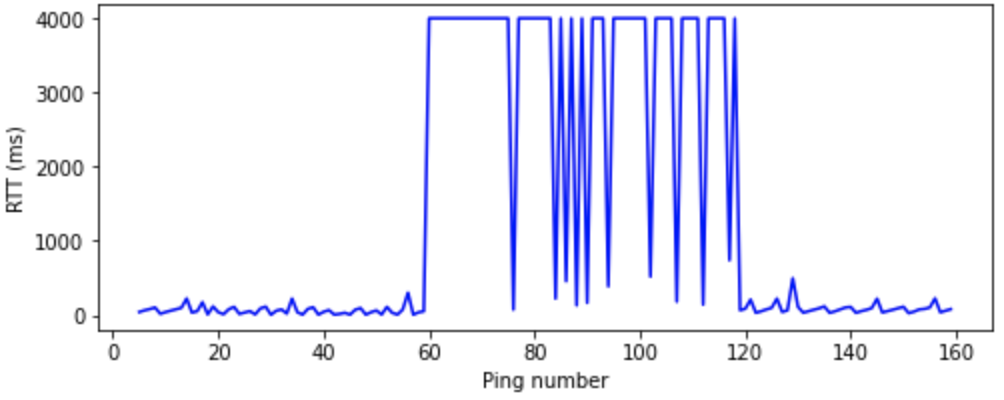
\includegraphics[width=5.8cm]{./ping/ping-rtt1.png} }}%
    \qquad
    \subfloat[\centering The pinged device is the target. The attack has been performed by one attacker, 1 thread, rr any]{{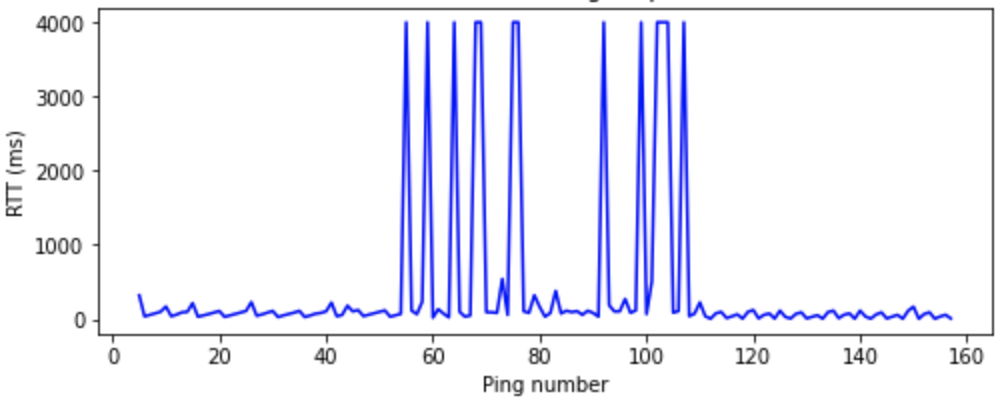
\includegraphics[width=5.8cm]{./ping/ping-rtt2.png} }}%
    \caption{Ping RTTs time series examples}%
    \label{fig:rtts-time-series}%
\end{figure}

\begin{figure}[H]
	\centering
    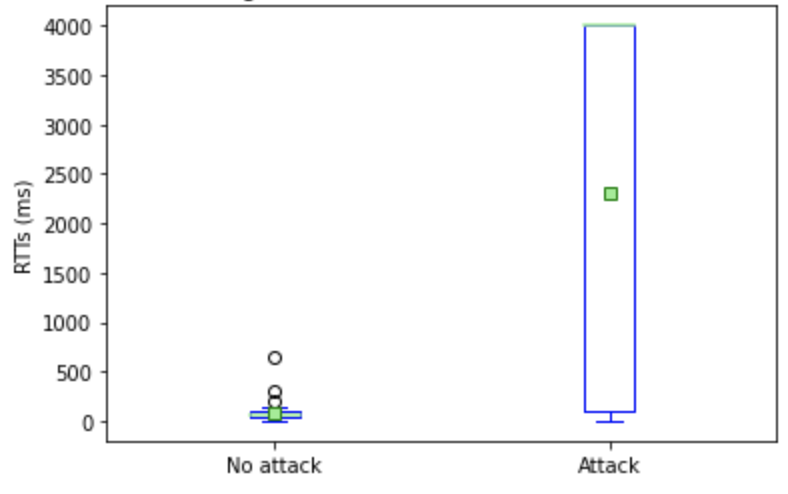
\includegraphics[width=\linewidth]{./ping/ping-boxplot1.png}
    \caption{Boxplots - Ping RTTs vs network condition}
	\label{fig:ping-boxplot1}%
\end{figure}

But how it can be ensured that the mean effect of the two groups of samples (attack, no attack) is different not just visually but also statistically\mbox{?}

A useful statistical test that can help to perform this kind of analysis is the {\it{Mann-Whitney U Test}}, explained below. \newline

By performing the mentioned test, it can be noticed, in figure \ref{fig:mannwhitneyu1}, that the two samples have very different means, and it is statistically significant (small p-value).

\begin{figure}[H]\centering
    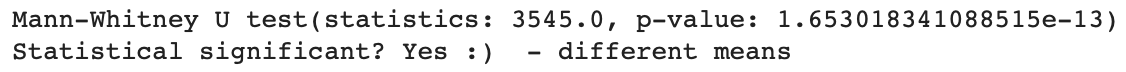
\includegraphics[width=\linewidth]{./ping/mannwhitneyu1.png}
    \caption{Mann-Whitney U Test results}
	\label{fig:mannwhitneyu1}
\end{figure}

\subparagraph{Mann-Whitney U Test \cite{MannWhitneyU}}
This statistical test does not assume that the distribution that have generated the different samples is normal.
In addition, the two samples does not must have the same length.

The null hypothesis is that the two groups have the same distribution, while the alternative hypothesis is that one group has larger (or smaller) values than the other.\\

Whereas, by distinguishing the different types of attacks, figure \ref{fig:ping-boxplot2}, other considerations can be extracted.

\begin{figure}[H]\centering
    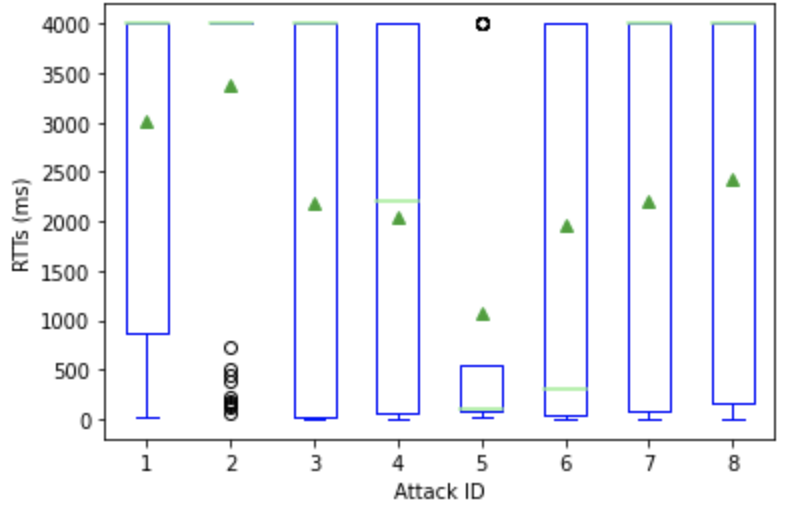
\includegraphics[width=\linewidth]{./ping/ping-boxplot2.png}
    \caption{Boxplots - Ping RTTs vs attack type}
	\label{fig:ping-boxplot2}
\end{figure}
Each of the attacks' id corresponds to a particular conducted experiment, as described in table \ref{tab:ping-attack-ids-descr}.

\begin{table}[H]
	\centering
	\begin{tabular}{|C{1.1cm}|C{1.5cm}|C{1.8cm}|C{0.5cm}|C{1.1cm}|}
		\hline
		\textbf{Attack ID} & \textbf{Attackers} & \textbf{Threads/ Attackers} & \textbf{RR} & \textbf{Pinged device} \\
		\hline
		\hline
		1 & 2 & 300 & any & another \\
		\hline
		2 & 2 & 300 & any & target \\
		\hline
		3 & 1 & 300 & any & target \\
		\hline
		4 & 1 & 10 & any & target \\
		\hline
		5 & 1 & 1 & any & target \\
		\hline
		6 & 1 & 100 & any & target \\
		\hline
		7 & 1 & 300 & a & target \\
		\hline
		8 & 1 & 300 & ptr & target \\
		\hline
	\end{tabular}
	\caption{mDNS attacks ID description}
	\label{tab:ping-attack-ids-descr}
\end{table}

From the boxplots in figure \ref{fig:ping-boxplot2}, it can be noticed that the worst condition has been obtained by using two attackers, with lots of active threads, and pinging the target device.

Finally, by changing the type of query performed the RTT changes, but not so much and so it cannot be said that changing the resource record does change the effect of the attack (random sampling).

It can be noticed that the attack causes problems not only to the target device, but even to other nodes connected within its network  (as shown in the boxplot correspondent to {\it{pinged device: another}}).
\subsection{mDNS probing results}
This section is focused on analyzing the effect size of the DoS attack over the mDNS protocol, and so consequentially the UDP, since mDNS works on top of UDP as already pointed out.

Different attacks have been performed, by changing the hyperparameter of the {\it{scripton}} code.

The expected behavior is that the effect of the DoS over the mDNS service is even worse with respect to the ICMP protocol case (ping).

The script used to generate the mDNS queries has already been discussed in the section \ref{sec:query-mdns-script}.
\paragraph{Time series}\mbox{}\\
Figure \ref{fig:mdns-rtts-time-series} shows the timeline of the mDNS queries RTTs when some particular kind of attacks have been performed.

\begin{figure}[H]
    \centering
    \subfloat[\centering The mDNS queried device is the target. The attack has been performed by one attacker, 300 threads, rr ptr]{{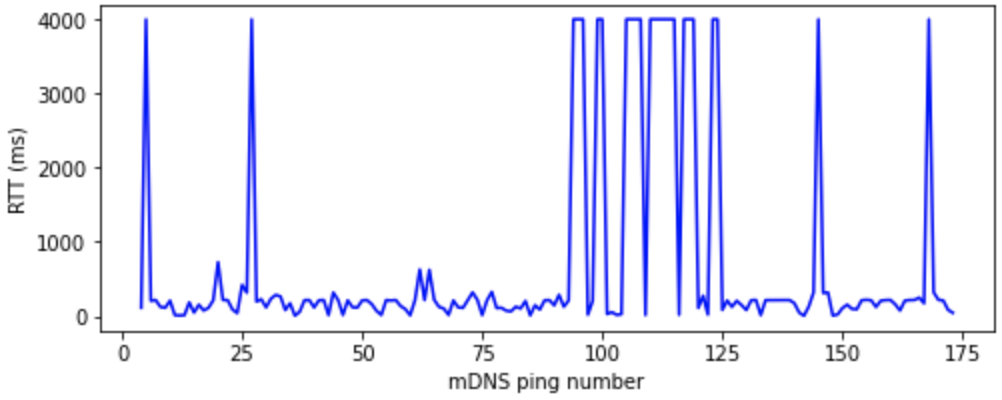
\includegraphics[width=5.8cm]{./mdns/mdnsping-rtt1.png} }}%
    \qquad
    \subfloat[\centering The mDNS queried device is another node connected within the same network of the target device. The attack has been performed by one attacker, 300 threads, rr any]{{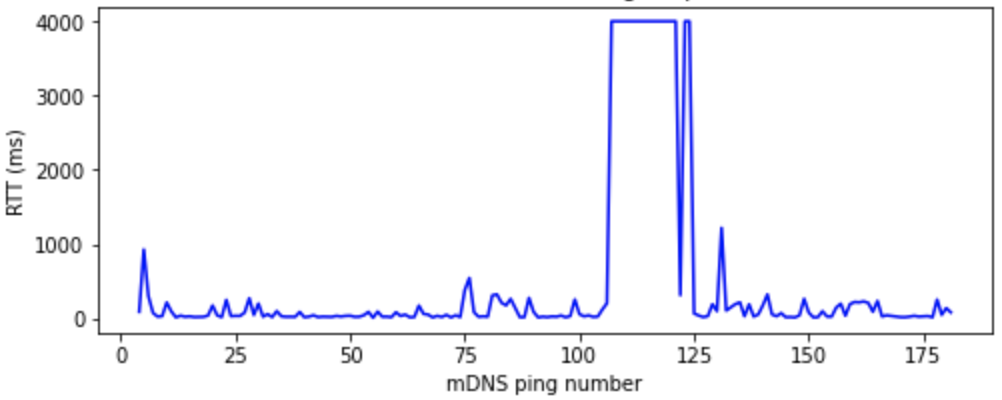
\includegraphics[width=5.8cm]{./mdns/mdnsping-rtt2.png} }}%
    \caption{mDNS queries RTTs time series examples}%
    \label{fig:mdns-rtts-time-series}%
\end{figure}

The same information is represented in a more compact way by the boxplots represented in the figure \ref{fig:mdns-boxplot2}.

In this case, since some single timeouts are present even when the attack is not performed, the attack starts when two timeouts are occurring one immediately after another. 

\paragraph{Boxplots}\mbox{}\\
This part is focused on analyzing the differences of the mDNS queries RTTs when the system was under attack and when not.

As illustrated in the following figure it can be noticed that the RTTs when the system was under attack, on average, are lower with respect the system under attack.
The reasoning is the same of the ping case of study.

\begin{figure}\centering
    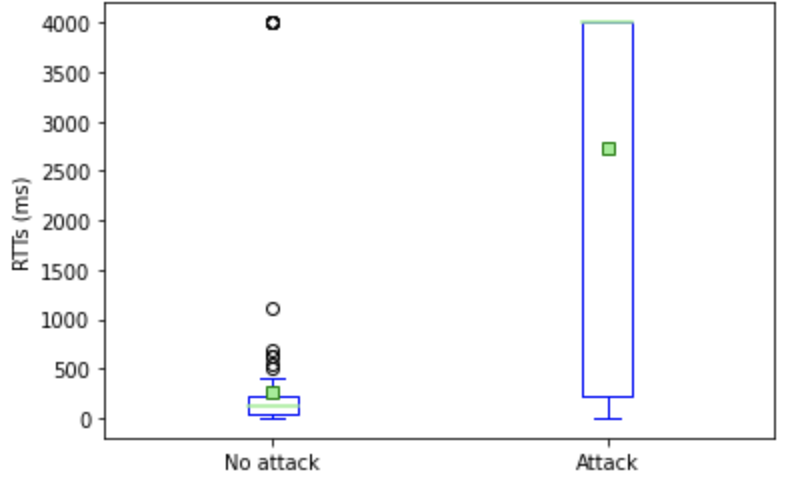
\includegraphics[width=\linewidth]{./mdns/mdns-boxplot1.png}
    \caption{Boxplots - mDNS queries RTTs vs network condition}
	\label{fig:mdns-boxplot1}
\end{figure}

Since more timeouts are occurring when the system is not under attack, the RTTs mean is slightly higher with respect to the ping case (when the network is not under attack).

By performing the Mann-Whitney U statistical test already discussed, the results in figure \ref{fig:mannwhitneyu2} are obtained.
\begin{figure}[H]\centering
    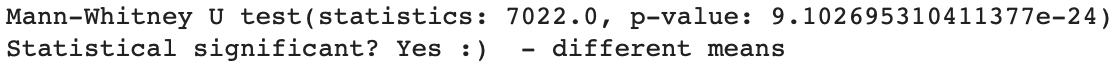
\includegraphics[width=\linewidth]{./mdns/mannwhitneyu2.png}
    \caption{Mann-Whitney U Test results}
	\label{fig:mannwhitneyu2}
\end{figure}

From this test it can be said that the two samples (no attack, attack) have different means and it is statistically significant (small p-value).

Furthermore, by comparing the statistics values in the figures \ref{fig:mannwhitneyu1} and \ref{fig:mannwhitneyu2} it can be seen that the effect of the DoS attack over the mDNS protocol is higher with respect to the case of the ICMP protocol. \newline

Now, different types of attacks will be distinguished, figure \ref{fig:mdns-boxplot2}, so that other considerations can be extracted.

Each of the attacks' id corresponds to a particular conducted experiment, as described in the table \ref{tab:mdns-ping-attack-ids-descr}.

Also here, by increasing the number of attackers the effect of the attack increases and so more timeouts occurs.

As strange result is that by increasing the number of threads and so exploiting more calculation power of the single device performing the attack, the order of magnitude of the attack decreases. \newline

Finally, by changing the type of query performed the RTT changes, but not so much and so it cannot be said that changing the resource record does change the effect of the attack (random sampling).

It can be noticed that the attack causes problems not only to the target device, but even to other nodes connected within its network.

It looks like the other nodes connected within the network of the attacked device have higher mDNS queries RTTs when the attack is performed, with respect to the target device.

\begin{figure}[H]
	\centering
    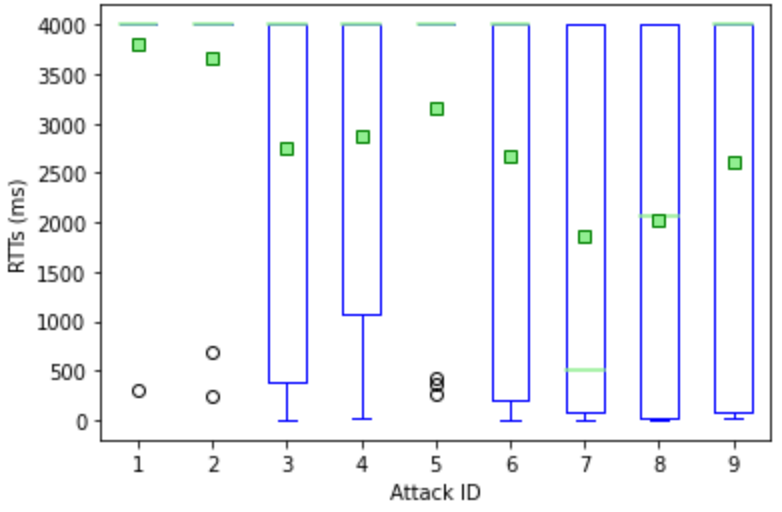
\includegraphics[width=\linewidth]{./mdns/mdns-boxplot2.png}
    \caption{Boxplots - mDNS queries RTTs vs attack type}
	\label{fig:mdns-boxplot2}
\end{figure}

\begin{table}[h]
	\centering
	\begin{tabular}{|C{1.1cm}|C{1.5cm}|C{1.8cm}|C{0.5cm}|C{1.1cm}|}
		\hline
		\textbf{Attack ID} & \textbf{Attackers} & \textbf{Threads/ Attackers} & \textbf{RR} & \textbf{mDNS queried device} \\
		\hline
		\hline
		1 & 1 & 300 & any & another \\
		\hline
		2 & 2 & 300 & any & another \\
		\hline
		3 & 1 & 300 & any & target \\
		\hline
		4 & 2 & 300 & any & target \\
		\hline
		5 & 1 & 1 & any & target \\
		\hline
		6 & 1 & 10 & any & target \\
		\hline
		7 & 1 & 100 & any & target \\
		\hline
		8 & 1 & 300 & a & target \\
		\hline
		9 & 1 & 300 & ptr & target \\
		\hline
	\end{tabular}
	\caption{mDNS attacks ID description}
	\label{tab:mdns-ping-attack-ids-descr}
\end{table}

%----------------------------------------------------------------------------------------
%	COUNTERMEASURES
%----------------------------------------------------------------------------------------

\section{Countermeasures} %se ci proviamo va bene qua altrimenti spostare in un'altra sezione
Unfortunately, mDNS does not provide any built-in security feature \cite{securityOfIoT}.
But how can be possible mitigate these kinds of DoS (or DDoS) attacks, based on mDNS protocol?

There are some specific countermeasures that can be applied to make the protocol more reliable and secure, and they can be considered as belonging in two mainly different categories:
\begin{itemize}[leftmargin=*]
	\item {\it{Simple methods}}: provided by operating systems
 	\item {\it{Sophisticated methods}}: provided by the services built on top of mDNS
\end{itemize}

\paragraph{Simple mitigation techniques}\mbox{}\\
Those kind of solutions can be implemented, for example, either {\it{disabling mDNS services}} when not needed, or
{\it{disabling the mDNS UDP port}} (5353) to block the traffic from/to outside the LAN (firewall).

In the majority of cases, mDNS protocol is enabled by default on most devices, but users might not be aware of this protocol running on their devices.

A possible cause of this DoS attack is that mDNS service, although designed for LAN, can be accessible from the Internet (so the botnet devices can start the attack from outside).

Different operating systems have implemented their own way to block the mDNS traffic. This is the case of Windows \cite{blockWindowsMDNS}  (after version 10); or Mac OS and Linux \cite{blockMacOsLinuxMDNS}.

\paragraph{Sophisticated mitigation techniques}\mbox{}\\
These methods, instead, are based on ensuring the following two security requirements: {\it{authenticity}}, and {\it{confidentiality}}.

The main goal of authenticity is to allow mDNS requests/responses, to only authenticated users, so that the hostnames are more difficult to be spoofed \cite{Bai2016StayingSA, Bai2017AppleZH, WuTSB16}.

Whereas, confidentiality (so the disclosure of informations) can be ensured by encrypting the mDNS traffic, to avoid that an user that has access to the network (or a man in the middle) can steal sensitive informations of other users devices \cite{Kaiser2014AddingPT, EfficientmDNS}.
%----------------------------------------------------------------------------------------
%	MITIGATION/PREVENTION
%----------------------------------------------------------------------------------------

\section{Other vulnerabilities}
The mDNS protocol does not provide any security services, such as DNSSEC or DNS over TLS for the well-known DNS protocol, since they are difficult to configure in small and simple local area networks. 

This is why local networks using this protocol may be subject to security threats. 

Analyzing all the vulnerabilities of services/products using the mDNS protocol, it appears that they can be categorized into four main types of threats:
\begin{itemize}[leftmargin=*]
	\item {\it{denial of service attack}}: where attackers fill the local network nodes (with mDNS enabled) with lots of messages that exploit protocol-specific features. These messages can make nodes unreachable and overload the local network
	\item {\it{sensitive information leak}}: where attackers can be able to enter the local network and obtain sensitive information
	\item {\it{remote code execution}}: where attackers can access a computer in the local area network and can execute system commands, write, modify, delete, or read files
	\item {\it{buffer overflow}}: where attackers manipulate the software code to carry out malicious actions and compromise the affected system 
\end{itemize}

\paragraph{Denial of Service}\mbox{}\\
DoS attacks are caused by lot of vulnerabilities (e.g. CVE-2021-1439 \cite{CVE-2021-1439}) in which insufficient checks are made on incoming mDNS messages.
But also by other vulnerabilities in which devices are misconfigured and inadvertently respond to unicast queries with source addresses that are not link-local. 

For example, the vulnerability CVE-2017-6520 \cite{CVE-2017-6520} affects the mDNS responder in the BOSE Soundtouch 30 series. They inadvertently respond to IPv4 unicast queries with source addresses that are not link-local. According to the RFC 6762\cite{rfc6762} section 5.5, "Since it is possible for a unicast query to be received from a machine outside the local link, responders should check that the source address in the query packet matches the local subnet for that link (or, in the case of IPv6, the source address has an on-link prefix) and silently ignore the packet if not." \newline\newline
It should also be added that the nature of the protocol, in which multicast queries are involved, is itself a feature that attackers can exploit to carry out a DoS/DDoS attack on a local network after gaining access to it.

\paragraph{Sensitive information leak}\mbox{}\\
In analyzing the vulnerabilities of this protocol, it is observed that leakage of sensitive information, but more generally of any information one does not want to share, is caused by several factors. Again, the most frequent problem, evidenced by many vulnerabilities is caused by malconfigurations that allow devices to respond to mDNS queries not coming from within the local network. 

Another vulnerability (CVE-2020-3182 \cite{CVE-2020-3182}) that plagues the protocol configuration of Cisco Webex Meetings Client for macOS, exists because some sensitive information is included in the mDNS replies. Thus an attacker could exploit this vulnerability by making mDNS queries for a particular service against an affected device, and gain access to sensitive information. A similar problem is highlighted by another vulnerability (CVE-2020-26966 \cite{CVE-2020-26966}), in which searching for a single word from the address bar causes an mDNS query to be sent on the local network searching for a hostname consisting of that string (affects Firefox $<$ 83, Firefox ESR $<$ 78.5, and Thunderbird $<$ 78.5 on Windows operating systems). Thus allowing anyone connected to the local network to obtain this data.
\paragraph{Remote code execution}\mbox{}\\
Remote code execution is a threat highlighted by some vulnerabilities where there are errors in checking some return values of certain functions. 

The CVE-2020-6072 {\cite{CVE-2020-6072}} vulnerability evinces that the minimal mDNS resolver library named \textit{libmicrodns} \cite{libmicrodns} in version 0.1.0, when parsing compressed labels in mDNS messages, does not check the return value of a function. Similar problem is the one highlighted in vulnerability CVE-2014-9378 \cite{CVE-2014-9378} in which the free and open source network security tool for man-in-the-middle attacks on a LAN, named \textit{Ettercap} \cite{Ettercap}, does not validate certain return values.
\newline
By not checking the return values of certain functions, the attackers can execute malicious code remotely. 

\paragraph{Buffer overflow}\mbox{}\\
A buffer overflow condition exists when a program attempts to put more data in a buffer than it can hold or when a program attempts to put data in a memory area past a buffer. Writing outside the bounds of a block of allocated memory can corrupt data, crash the program, or cause the execution of malicious code. The buffer overflow exploit techniques a hacker uses depends on the architecture and operating system being used by their target. However, the additional data that are sent to a program will probably contain malicious code that allows the attacker to perform additional actions and send new instructions to the application. 

There are some vulnerabilities (e.g. CVE-2015-7987 \cite{CVE-2015-7987}) that highlight buffer overflow problems. In particular, vulnerabilities CVE-2015-7987 \cite{CVE-2015-7987} and CVE-2007-2386 \cite{CVE-2007-2386} evince these problems for
\textit{mDNSResponder} the core Bonjour's process that regularly scans the local network looking for other Bonjour-enabled devices. Note that Apple's Bonjour service is available for both Mac OS and Windows.  

%----------------------------------------------------------------------------------------
%	MITIGATION/PREVENTION
%----------------------------------------------------------------------------------------
\section{Conclusions}
This report presented an overview of the field of IT security, in particular it touched a particular problem: the DoS (or DDoS) attacks performed on top of mDNS. \newline
More in detail the following topics have been covered:
\begin{itemize}[leftmargin=*]
	\item what are the DoS attacks and which are the objective of performing them 
	\item the mDNS protocol, its working principles, how to exploit its vulnerabilities to perform a Dos (or DDoS) attack, and some possible 
		  countermeasures to overcome the security issues
 	\item how to exploit mDNS specification to implement a script that can be used in order to perform mDNS DoS attacks
 	\item how to implement a script to measure the mDNS ping statistics
	\item some active and passive monitoring tools that can be used to analyze the traffic over the network,
	      to avoid that the effects become worse and worse over time
 	\item a discussion on the obtained results, supported by the use of statistics and some visualization tools
\end{itemize}

Many other aspects can be extended, such as the implementation of a solution that mitigates the effects of DoS attacks over mDNS, using preventive actions 
(for example blocking the working of the protocol when the traffic on the network, using the latter, becomes too high).
Furthermore, the other treated vulnerabilities can be studied and possible countermeasures can be proposed.

\paragraph{Legal issues \cite{IllegalIssues}} The code to carry out the attack was used on a test network. If you want to use it, talk to the network administrator, because DoS attacks are illegal and large fines, accompanied by years in prison, belong to malicious users.

%----------------------------------------------------------------------------------------
%	REFERENCE LIST
%----------------------------------------------------------------------------------------
\clearpage
\phantomsection
\bibliographystyle{unsrt}
\bibliography{mybibl.bib}

%----------------------------------------------------------------------------------------

\end{document}